\section{Diagnóstico de Multicolinealidad}
\label{sec:multicolinealidad}

\todo{Pregunta aca: vale la pena hacer el analisis para cada sujeto?}

La presencia de multicolinealidad entre los predictores de un modelo 
de regresión puede inflar la varianza de los coeficientes estimados 
y dificultar su interpretación. Si bien la regresión Ridge mitiga 
este problema mediante la penalización $\lambda \|\beta\|^2$, que 
estabiliza los coeficientes en presencia de predictores correlacionados, 
no lo elimina completamente. Por esta 
razón, se realiza un diagnóstico de multicolinealidad previo al modelado 
de EEG, con el objetivo de identificar pares redundantes y fundamentar 
decisiones de descarte antes de incorporar las features al modelo.

Dado que varias features presentan distribuciones fuertemente sesgadas, 
como se documentó en el análisis distribucional 
(sección~\ref{sec:analisis_distribucional}), se empleó la correlación 
de Spearman en lugar de la de Pearson. La correlación de Spearman opera 
sobre los rangos de los datos y es robusta a outliers y a la no 
normalidad, lo que la hace más apropiada para el conjunto de features 
analizado.

La Figura~\ref{fig:heatmap_correlaciones} presenta la matriz de 
correlaciones de Spearman entre las 20 features candidatas, calculada 
sobre el pool completo de fijaciones ($N = 61.252$). Los colores rojos 
indican correlaciones positivas y los azules correlaciones negativas; 
las etiquetas de cada feature están coloreadas según su grupo de 
pertenencia.

\begin{figure}[H]
    \centering
    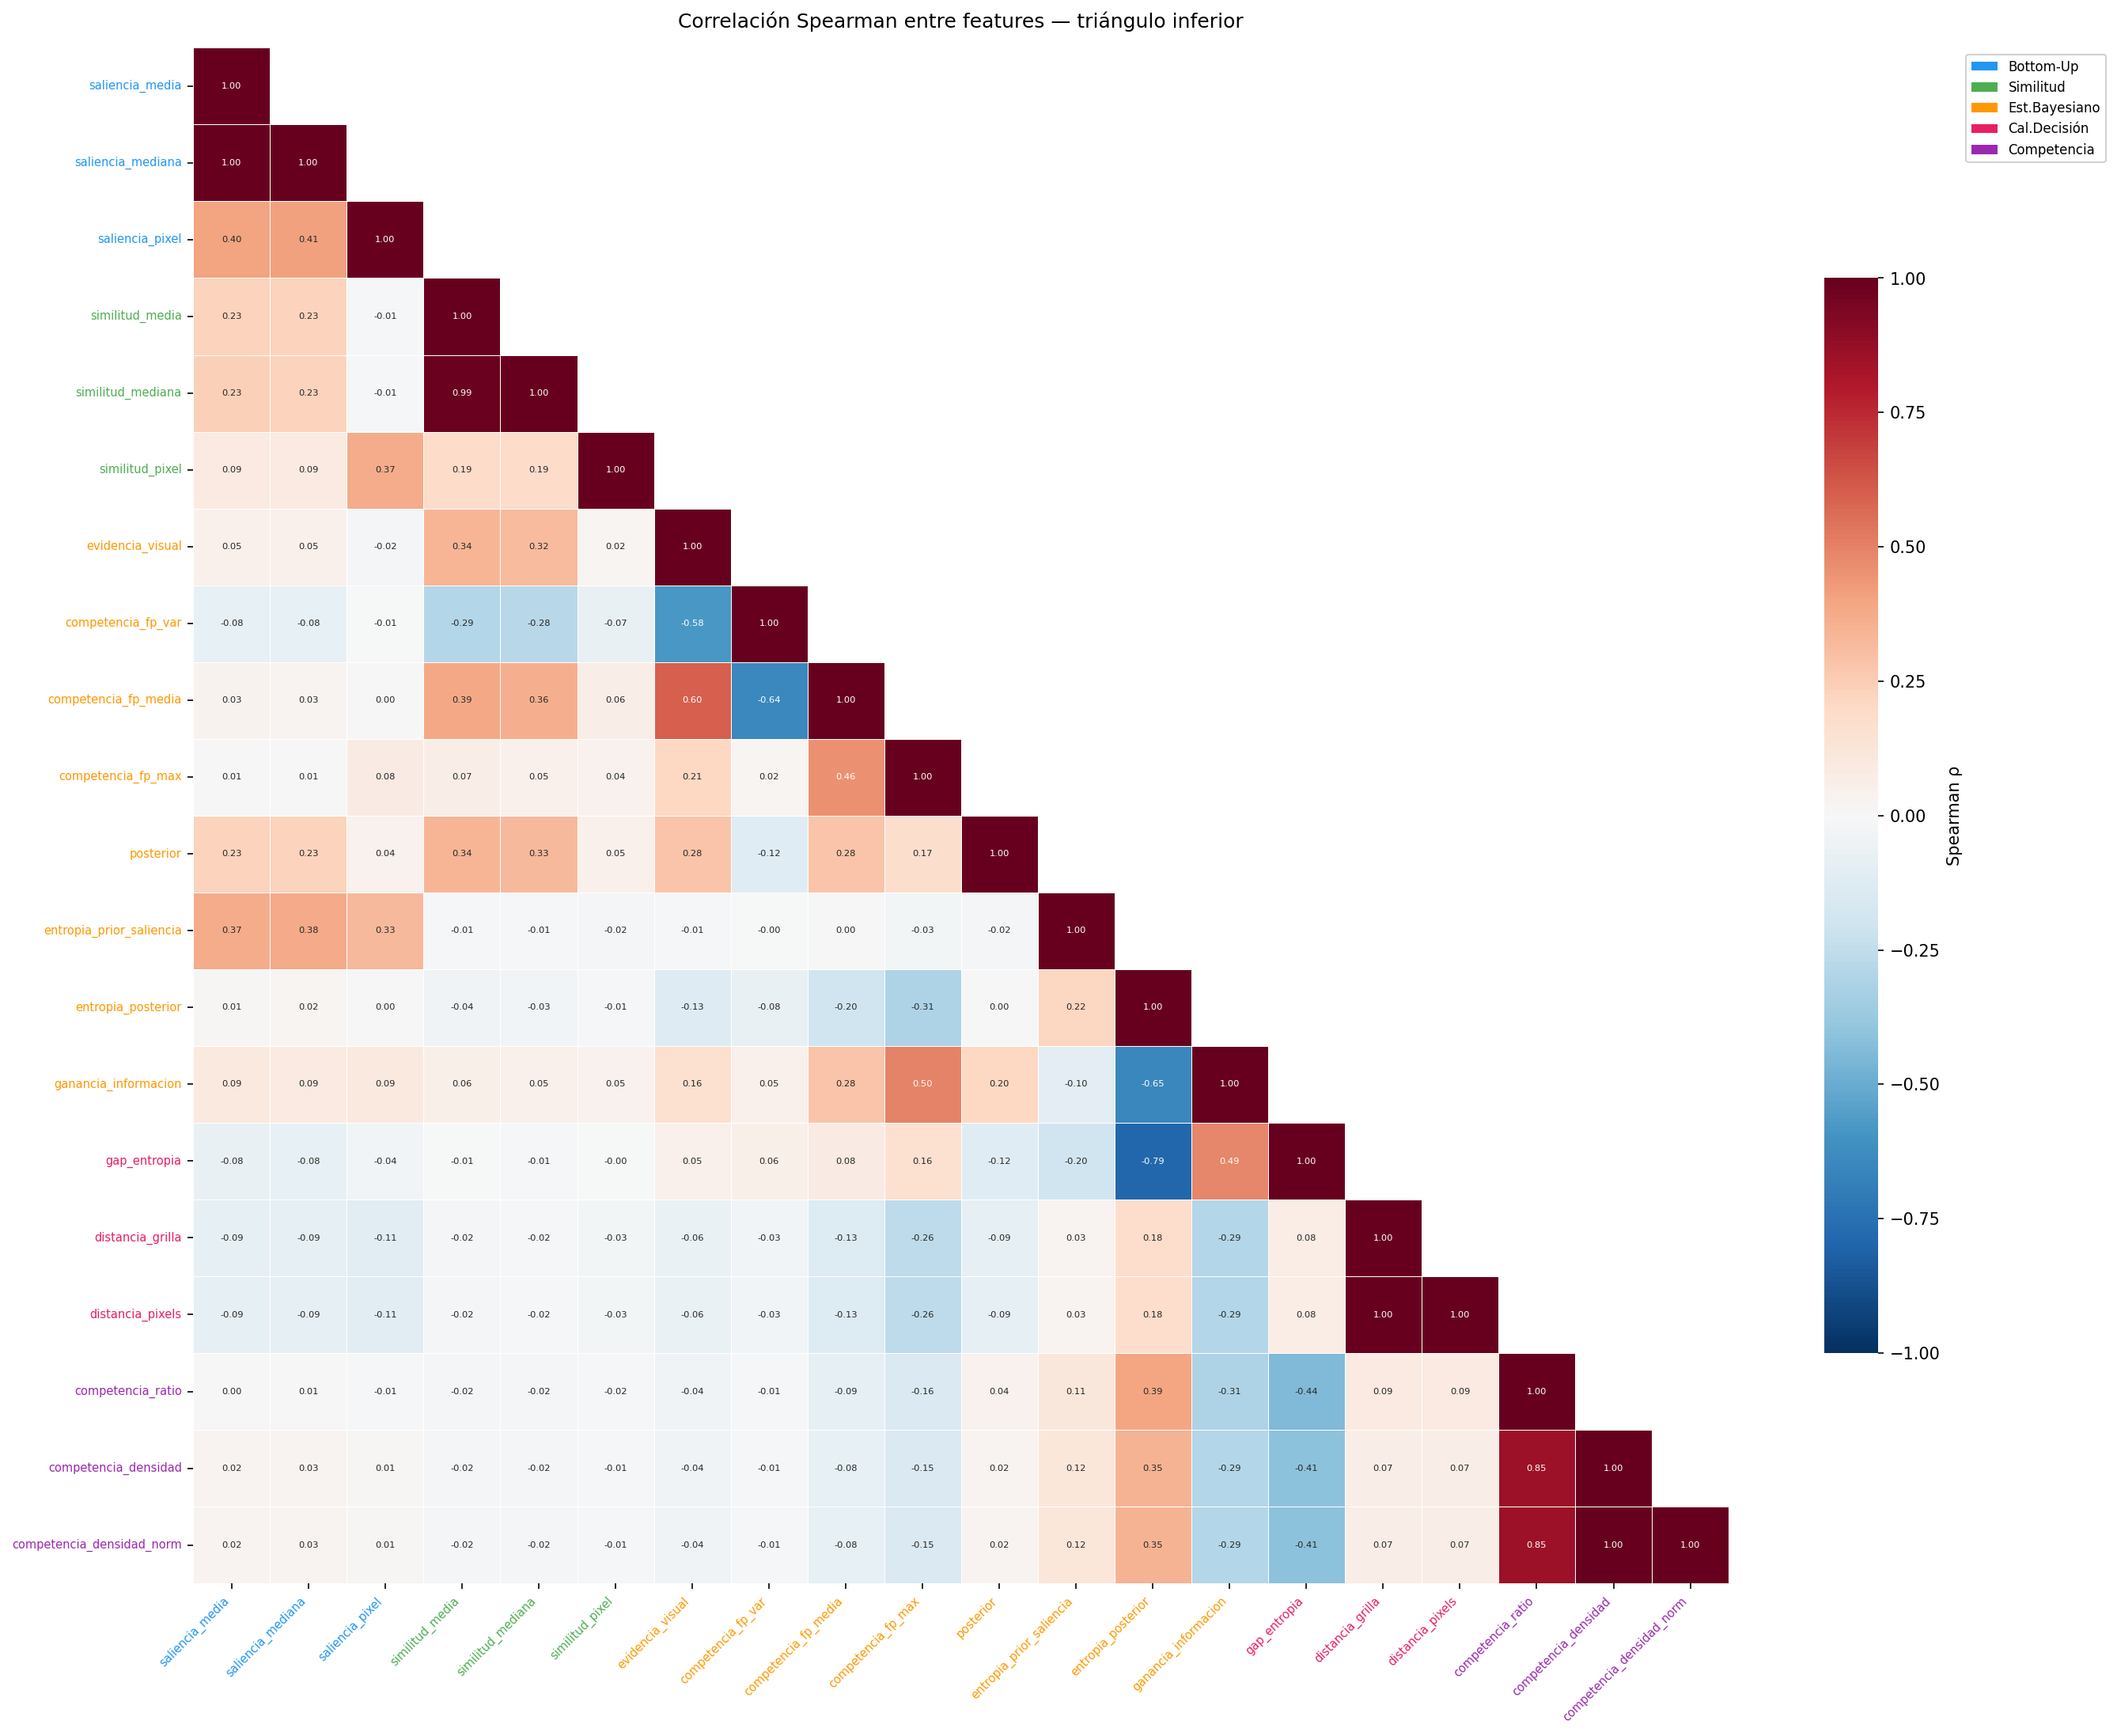
\includegraphics[width=\textwidth]{chapters/03_analisis_features/images/bloque5_corr_heatmap}
    \caption{Matriz de correlaciones de Spearman entre las features 
    candidatas. Los colores de las etiquetas indican el grupo de 
    pertenencia de cada feature.}
    \label{fig:heatmap_correlaciones}
\end{figure}

Se observan bloques de alta correlación 
intragrupo en Bottom-Up y Similitud: \texttt{saliencia\_media} y 
\texttt{saliencia\_mediana} presentan $\rho = 1.00$, y 
\texttt{similitud\_media} y \texttt{similitud\_mediana} presentan 
$\rho = 0.99$. Estas correlaciones son esperables dado que ambas 
features de cada par fueron diseñadas como resúmenes alternativos 
de la misma información espacial y se incluyeron por separado 
con el objetivo de evaluar su performance individual en el modelo. 
Lo mismo ocurre dentro del grupo de Competencia: 
\texttt{competencia\_densidad} y \texttt{competencia\_densidad\_norm} 
presentan $\rho = 1.00$ por ser transformaciones lineales entre sí, 
y ambas muestran una correlación moderada con 
\texttt{competencia\_ratio} ($\rho = 0.85$), también esperable dado 
que las tres cuantifican distintos aspectos de la misma estructura 
del mapa EIG.

En segundo lugar, se observan correlaciones altas entre grupos que 
no fueron anticipadas en el diseño de las features. 
\texttt{entropia\_posterior} y \texttt{gap\_entropia} presentan 
una correlación negativa de $\rho = -0.79$, y 
\texttt{ganancia\_informacion} y \texttt{gap\_entropia} presentan 
una correlación positiva de $\rho = 0.69$. 

